%%%%%%%%%%%%%%%%%%%%%%%%%%%%%%%%%%%%%%%%%%%%%%%%%%%%%%%%%%%%%%%%%%%%%%%%
\chapter{Data} \label{chap:Data}
%%%%%%%%%%%%%%%%%%%%%%%%%%%%%%%%%%%%%%%%%%%%%%%%%%%%%%%%%%%%%%%%%%%%%%%%
\vspace{1cm}

% Type here an introduction to the chapter

\section{Kispi}
The Kispi dataset\,\cite{FeTA_MICCAI} originates from the University Children's Hospital Zurich, Switzerland, in the context of the FeTA challenge. All data were acquired with institutional ethics committee approval from the Canton of Zurich, with research consent provided by the mothers for the use of their data. The dataset is open-source and fully anonymized\,\cite{FeTA2024_paper}.

The Kispi cohort comprises fetal brain MRI scans from subjects with both normal and pathological neurodevelopment. The pathological cases include a variety of congenital disorders, such as spina bifida and ventriculomegaly, reflecting a clinically relevant population\,\cite{FeTA2024_paper, Ciceri2024}. The dataset spans a gestational age (GA) range of approximately 20 to 35 weeks. For the FeTA 2024 challenge, the Kispi data was partitioned into a training set of 80 volumes and a test set of 40 volumes, but only the training set is publicly available. The training partition consists of 31 neurotypical and 49 pathological cases\,\cite{FeTA2024_review}.

All imaging was performed on 1.5\,T and 3\,T GE Signa Discovery (MR450 and MR750) whole-body scanners. The acquisitions were conducted without the use of maternal or fetal sedation. Depending on the specific case, either an 8-channel cardiac coil or a standard body coil was employed\,\cite{FeTA2024_paper}.

The acquisition protocol consisted of T2-weighted single-shot fast spin echo (\textsc{ssfse}) sequences acquired in the axial, coronal, and sagittal planes relative to the fetal brain. Key sequence parameters were maintained as follows\,\cite{FeTA2024_paper}:
\begin{itemize}
    \item \textbf{Repetition Time (TR):} 2000--3500\,ms.
    \item \textbf{Echo Time (TE):} 120\,ms (minimum).
    \item \textbf{Flip Angle:} 90 degrees.
    \item \textbf{Acquisition Resolution:} An in-plane resolution of $0.5 \times 0.5$\,mm with a slice thickness ranging from 3 to 5\,mm was employed.
    \item \textbf{Field of View (FOV) and Matrix Size:} The FOV (200--240\,mm) and image matrix (1.5\,T: $256 \times 224$; 3\,T: $320 \times 224$) were adjusted according to the GA and size of the fetus.
\end{itemize}

Prior to reconstruction, all acquired images for a given subject underwent a manual quality review to compile a stack of suitable scans, with at least one brain scan in each orientation. Each image stack was then reoriented to a standard anatomical plane, and a semi-automated method was used to generate the masks of the single labels in the fetal brain. Segmentations were then inspected and refined. Following these pre-processing steps, the data were processed using one of two distinct SR reconstruction pipelines, resulting in two sub-cohorts within the Kispi dataset. The parcellation used distinguishes 7 labels: external cerebrospinal fluid (CSF), cortical gray matter (cGM), white matter (WM), ventricles (including cavum), cerebellum, deep gray matter (dGM), and brainstem (BS)\,\cite{FeTA2024_paper}.

40 image stacks, that is, half of the available Kispi stacks, was processed using the \textsc{mial} Super-Resolution Toolkit (\textsc{mialsrtk}) pipeline\,\cite{Tourbier2015, MIALSRTK}. The resulting 3D volumes for this sub-cohort have an isotropic resolution of $0.5 \times 0.5 \times 0.5$\,mm. The remaining 40 stacks were reconstructed using a pipeline based on the Image Registration Toolkit (\textsc{irtk})\,\cite{Kuklisova2012, irtk-simple}. The reconstructions from this pipeline yielded 3D volumes with an isotropic resolution of $1.0 \times 1.0 \times 1.0$\,mm\,\cite{FeTA2024_review}. However, scans from both SRR methods were standardised to $256 \times 256 \times 256$ voxels. More information about the SR reconstruction algorithms is provided in Section \ref{sec:SuperResolutionReconstruction}. Data aforementioned are collected in Tab.\,\ref{tab:datasets}.

\begin{figure}[htbp]
    \centering
    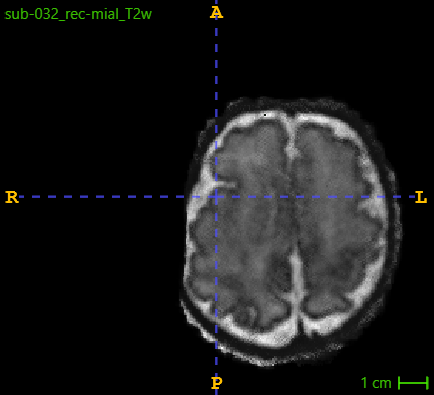
\includegraphics[width=0.35\textwidth]{figures/mial_1.png} \quad
    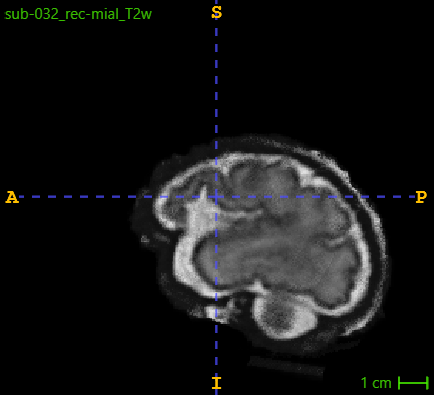
\includegraphics[width=0.35\textwidth]{figures/mial_2.png} \\
    \vspace{10pt}
    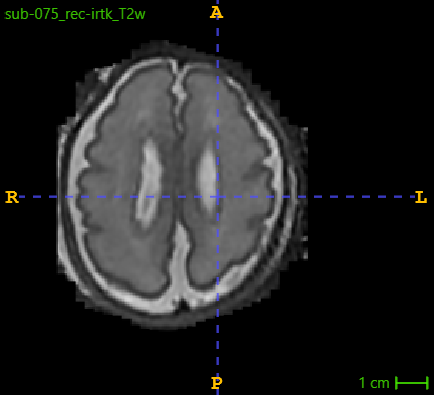
\includegraphics[width=0.35\textwidth]{figures/irtk_1.png} \quad
    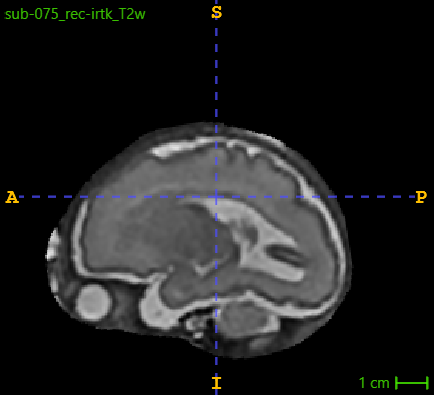
\includegraphics[width=0.35\textwidth]{figures/irtk_2.png}
    \caption{}
    \label{fig:kispi_images}
\end{figure}
\begin{figure}[htbp]
    \centering
    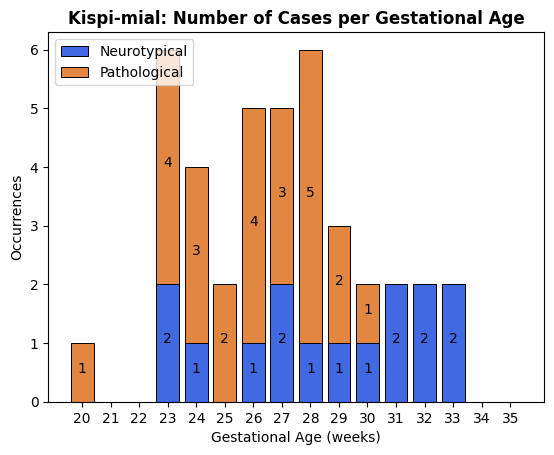
\includegraphics[width=0.45\textwidth]{figures/k-mial_GA.png} \quad
    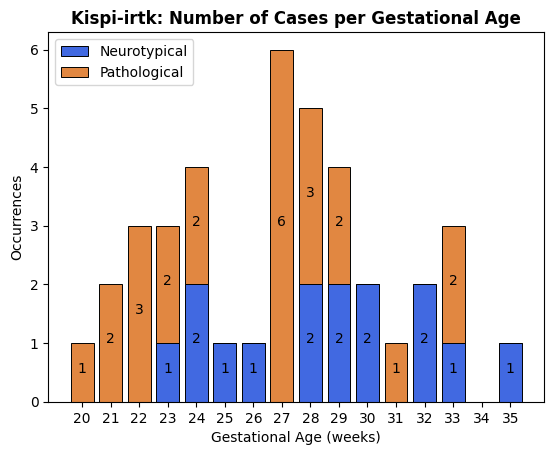
\includegraphics[width=0.45\textwidth]{figures/k-irtk_GA.png}\\
    \vspace{10pt}
    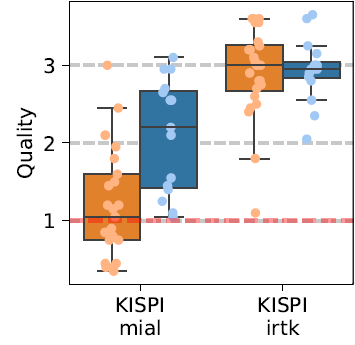
\includegraphics[width=0.35\textwidth]{figures/kispi_quality.png}
    \caption{}
    \label{fig:kispi_plots}
\end{figure}

\section{dHCP}

\begin{table}[htbp]
    \centering
    \begin{tabular}{c|c|c|c|c|c|c}
        \toprule
        \textbf{Name} & $\textbf{N}_\textbf{n}$\textbf{/}$\textbf{N}_\textbf{p}$ & \makecell{\textbf{GA range} \\ \textbf{(weeks)}} & \makecell{\textbf{Field} \\ \textbf{strength}} & \textbf{Scanner} & \textbf{SRR} & \textbf{Parcel.} \\ \midrule
        Kispi-mial & 15/25 & 20.0--32.8 & 1.5/3\,T* & \makecell{GE Signa \\ Discovery \\ MR450/750*} & \textsc{mialsrtk} & 7 labels \\ \hline
        Kispi-irtk & 16/24 & 20.01--34.8 & 1.5/3\,T* & \makecell{GE Signa \\ Discovery \\ MR450/750*} & \textsc{irtk} & 7 labels \\ \hline
        dHCP & 248/0 & 20.9--38.3 & 3\,T & \makecell{Philips \\ Achieva} & Cordero & 17 labels \\
        \bottomrule
    \end{tabular}
    \caption{Dataset properties. $\text{N}_\text{n}$ and $\text{N}_\text{p}$ respectively indicates the number of normal and pathological cases. *The field strengths respectively refers to the scanners.}
    \label{tab:datasets}
\end{table}

\section{Data Specifications}
